\section{Stubs}
\label{sec:Stubs}
%%%%%%%%%%%%%%%%%%%%%%%%%%%%%%%%%%%%%%%%%%%%%%%%%%%%%%%%
\begin{figure}[h!]
\begin{center}
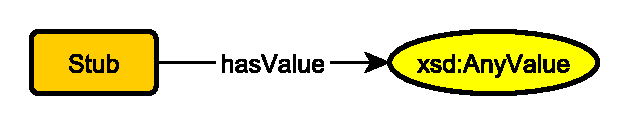
\includegraphics[width=.4\textwidth]{figures/stubs}
\end{center}
\caption{Schema Diagram for Stubs. The visual notation is explained in Chapter \ref{chap:prelims}.}
\label{fig:Stubs}
\end{figure}
\subsection{Summary}
\label{sum:Stubs}
%%%%%%%%%%%%%%%%%%%%%%%%%%%%
Stubs are a very minimal pattern that could also be described as a technique or best practice. Essentially, during modelling, there are frequently times when developers recognize that a concept is complex, but also out of the scope of an ontology or knowledge graph. However, the developer would like to keep the ontology extensible or allow others to build off of the ontology at that point. One example of this is Name or Title. In many cases, there is no reason to store more than a string for a name or title. However, names and titles are not necessarily inherent to a thing at all times. Yet, delving into those details may be unnecessary for a use-case. To account for this, a developer may want to use as stub. That is, acknowledge the complexity of a concept, but also include the information that is useful. This metapattern is described in more detail in \cite{stub}. 

%%%%%%%%%%%%%%%%%%%%%%%%%%%%%%%%%%%%%%%%%%%%%%%%%%%%%%%%
\subsection{Axiomatization}
\label{axs:Stubs}
%%%%%%%%%%%%%%%%%%%%%%%%%%%%
\begin{align}
\top &\sqsubseteq \textsf{hasValue.xsd:AnyValue}
\end{align}

%%%%%%%%%%%%%%%%%%%%%%%%%%%%%%%%%%%%%%%%%%%%%%%%%%%%%%%%
\subsection{Explanations}
\label{exp:Stubs}
%%%%%%%%%%%%%%%%%%%%%%%%%%%%
\begin{enumerate}
\item Range: the range of \textsf{hasValue} is any xsd datatype. We use AnyValue in the above axiom to indicate that any datatype will suffice.
\end{enumerate}

%%%%%%%%%%%%%%%%%%%%%%%%%%%%%%%%%%%%%%%%%%%%%%%%%%%%%%%%
\subsection{Competency Question}
\label{cqs:Stubs}
%%%%%%%%%%%%%%%%%%%%%%%%%%%%
\begin{enumerate}[CQ1.]
\item Which street is that?
\item What is the title of Alfred Tennyson?
\end{enumerate}

\newpage
%%%%%%%%%%%%%%%%%%%%%%%%%%%%%%%%%%%%%%%%%%%%%%%%%%%%%%%%
% End Section
%%%%%%%%%%%%%%%%%%%%%%%%%%%%%%%%%%%%%%%%%%%%%%%%%%%%%%%%
%%%%%%%%%%%%%%%%%%%%%%%%%%%%%%%%%%%%%%%%%%%%%%%%%%%%%%%%